\documentclass[12pt,letterpaper]{article}
\usepackage{graphicx,textcomp}
\usepackage{natbib}
\usepackage{setspace}
\usepackage{fullpage}
\usepackage{color}
\usepackage[reqno]{amsmath}
\usepackage{amsthm}
\usepackage{fancyvrb}
\usepackage{amssymb,enumerate}
\usepackage[all]{xy}
\usepackage{endnotes}
\usepackage{lscape}
\newtheorem{com}{Comment}
\usepackage{float}
\usepackage{hyperref}
\newtheorem{lem} {Lemma}
\newtheorem{prop}{Proposition}
\newtheorem{thm}{Theorem}
\newtheorem{defn}{Definition}
\newtheorem{cor}{Corollary}
\newtheorem{obs}{Observation}
\usepackage[compact]{titlesec}
\usepackage{dcolumn}
\usepackage{tikz}
\usetikzlibrary{arrows}
\usepackage{multirow}
\usepackage{xcolor}
\newcolumntype{.}{D{.}{.}{-1}}
\newcolumntype{d}[1]{D{.}{.}{#1}}
\definecolor{light-gray}{gray}{0.65}
\usepackage{url}
\usepackage{listings}
\usepackage{color}

\definecolor{codegreen}{rgb}{0,0.6,0}
\definecolor{codegray}{rgb}{0.5,0.5,0.5}
\definecolor{codepurple}{rgb}{0.58,0,0.82}
\definecolor{backcolour}{rgb}{0.95,0.95,0.92}

\lstdefinestyle{mystyle}{
	backgroundcolor=\color{backcolour},   
	commentstyle=\color{codegreen},
	keywordstyle=\color{magenta},
	numberstyle=\tiny\color{codegray},
	stringstyle=\color{codepurple},
	basicstyle=\footnotesize,
	breakatwhitespace=false,         
	breaklines=true,                 
	captionpos=b,                    
	keepspaces=true,                 
	numbers=left,                    
	numbersep=5pt,                  
	showspaces=false,                
	showstringspaces=false,
	showtabs=false,                  
	tabsize=2
}
\lstset{style=mystyle}
\newcommand{\Sref}[1]{Section~\ref{#1}}
\newtheorem{hyp}{Hypothesis}

\title{Problem Set 1}
\date{Due: October 8, 2026}
\author{Ella Lang}

\begin{document}
	\maketitle
	
	\section*{Instructions}
	\begin{itemize}
	\item Please show your work! You may lose points by simply writing in the answer. If the problem requires you to execute commands in \texttt{R}, please include the code you used to get your answers. Please also include the \texttt{.R} file that contains your code. If you are not sure if work needs to be shown for a particular problem, please ask.
\item Your homework should be submitted electronically on GitHub.
\item This problem set is due before 23:59 on Thursday October 8, 2026. No late assignments will be accepted.
	\end{itemize}
	
	\vspace{1cm}
	\section*{Question 1: Education}

A school counselor was curious about the average of IQ of the students in her school and took a random sample of 25 students' IQ scores. The following is the data set:\\
\vspace{.5cm}

\lstinputlisting[language=R, firstline=36, lastline=36]{PS01_EL_LA.R}  


\vspace{1cm}

\begin{enumerate}
	\item Find a 90\% confidence interval for the average student IQ in the school (As a hint, you first need the mean and SD to create a CI):\\
	
 To calculate the confidence interval I used the formula: 
	\textit {mean +/- t-score * standard error.}
 The critical value was calculated through a t-distribution as n is under 30 and the standard deviation of the population is unknown. I first calculated the mean which was 98.44. To calculate the standard error I first calculated the standard deviation (13.09) using the sd() function, this was then divided by the square root of the length of y to get the standard error. I then calculated the critical value, which was 1.71, using the qt() function which provides a critical value from the t-distribution. I then plugged these values into the formula to find the lower and upper confidence intervals. \\
	
	\lstinputlisting[language=R, firstline=40, lastline=44]{PS01_EL_LA.R}  

	\lstinputlisting[language=R, firstline=49, lastline=49]{PS01_EL_LA.R}   
	
	\lstinputlisting[language=R, firstline=53, lastline=55]{PS01_EL_LA.R}  
	
	\noindent The 90 percent confidence interval is 93.96; 102.92. This means that we are 90 percent confident the true population mean falls within this interval, and that if this sample was repeated with other randomly selected groups, 90 percent of the sample means would contain the true population mean. \\
	
	\item Next, the school counselor was curious  whether  the average student IQ in her school is higher than the average IQ score (100) among all the schools in the country.\\ 
	\noindent Using the same sample, conduct the appropriate hypothesis test with $\alpha=0.05$.
	\vspace{.5cm}
	
	\noindent I conducted a one sample t-test to see if the sample mean was higher than the average IQ sore of 100. This t-test was one-tailed as the direction of the hypothesis is specified.  \\
	
	\noindent Null hypothesis: The sample IQ is less than or equal to the mean IQ of 100 among all the schools in the country. \\
	\noindent Alternative hypothesis: The sample IQ is higher than the mean IQ of 100 among all the schools in the country.  \\
	\lstinputlisting[language=R, firstline=59, lastline=59]{PS01_EL_LA.R}  
	
		\begin{verbatim} data:  y
			t = -0.59574, df = 24, p-value = 0.7215
			alternative hypothesis: true mean is greater than 100
			95 percent confidence interval:
			93.95993      Inf
			sample estimates:
			mean of x 
			98.44  \end{verbatim}

\end{enumerate}

\newpage
	
 \noindent The p-value 0.72 is also larger than the alpha of 0.05, so we fail to reject the null hypothesis that the sample IQ is less than or equal to the population mean IQ of 100. The t statistic is -0.596, showing a small difference between the sample and the population mean of 100. \\ 

	\section*{Question 2: Political Economy}

\noindent Researchers are curious about what affects the amount of money communities spend on addressing homelessness. The following variables constitute our data set about social welfare expenditures in the USA. \\
\vspace{.5cm}


\begin{tabular}{r|l}
	\texttt{State} &\emph{50 states in US} \\
	\texttt{Y} & \emph{per capita expenditure on shelters/housing assistance in state}\\
	\texttt{X1} &\emph{per capita personal income in state} \\
	\texttt{X2} &  \emph{Number of residents per 100,000 that are "financially insecure" in state}\\
	\texttt{X3} &  \emph{Number of people per thousand residing in urban areas in state} \\
	\texttt{Region} &  \emph{1=Northeast, 2= North Central, 3= South, 4=West} \\
\end{tabular}

\vspace{.5cm}
\noindent Explore the \texttt{expenditure} data set and import data into \texttt{R}.
\vspace{.5cm}
\lstinputlisting[language=R, firstline=65, lastline=67]{PS01_EL_LA.R}  
\vspace{.5cm}
\begin{itemize}

\item
Please plot the relationships among \emph{Y}, \emph{X1}, \emph{X2}, and \emph{X3}? What are the correlations among them (you just need to describe the graph and the relationships among them)? 

\lstinputlisting[language=R, firstline=74, lastline=78]{PS01_EL_LA.R}  

\noindent I used the GGally package to run the ggpairs function which creates a scatterplot matrix. The scatterplot matrix plots all variables against each other allowing for the visualization of any potential relationships between each of the variables. I also used the ggpairs function to display correlation coefficients to provide additional information about the strength and direction of the correlations between the variables. The distribution of each variable is also displayed in the plot. \\

\newpage

\begin{figure}[h!]\centering
	\caption{\footnotesize Scatterplots of Y, X1, X2, X3}
	\label{fig:plot_1}
	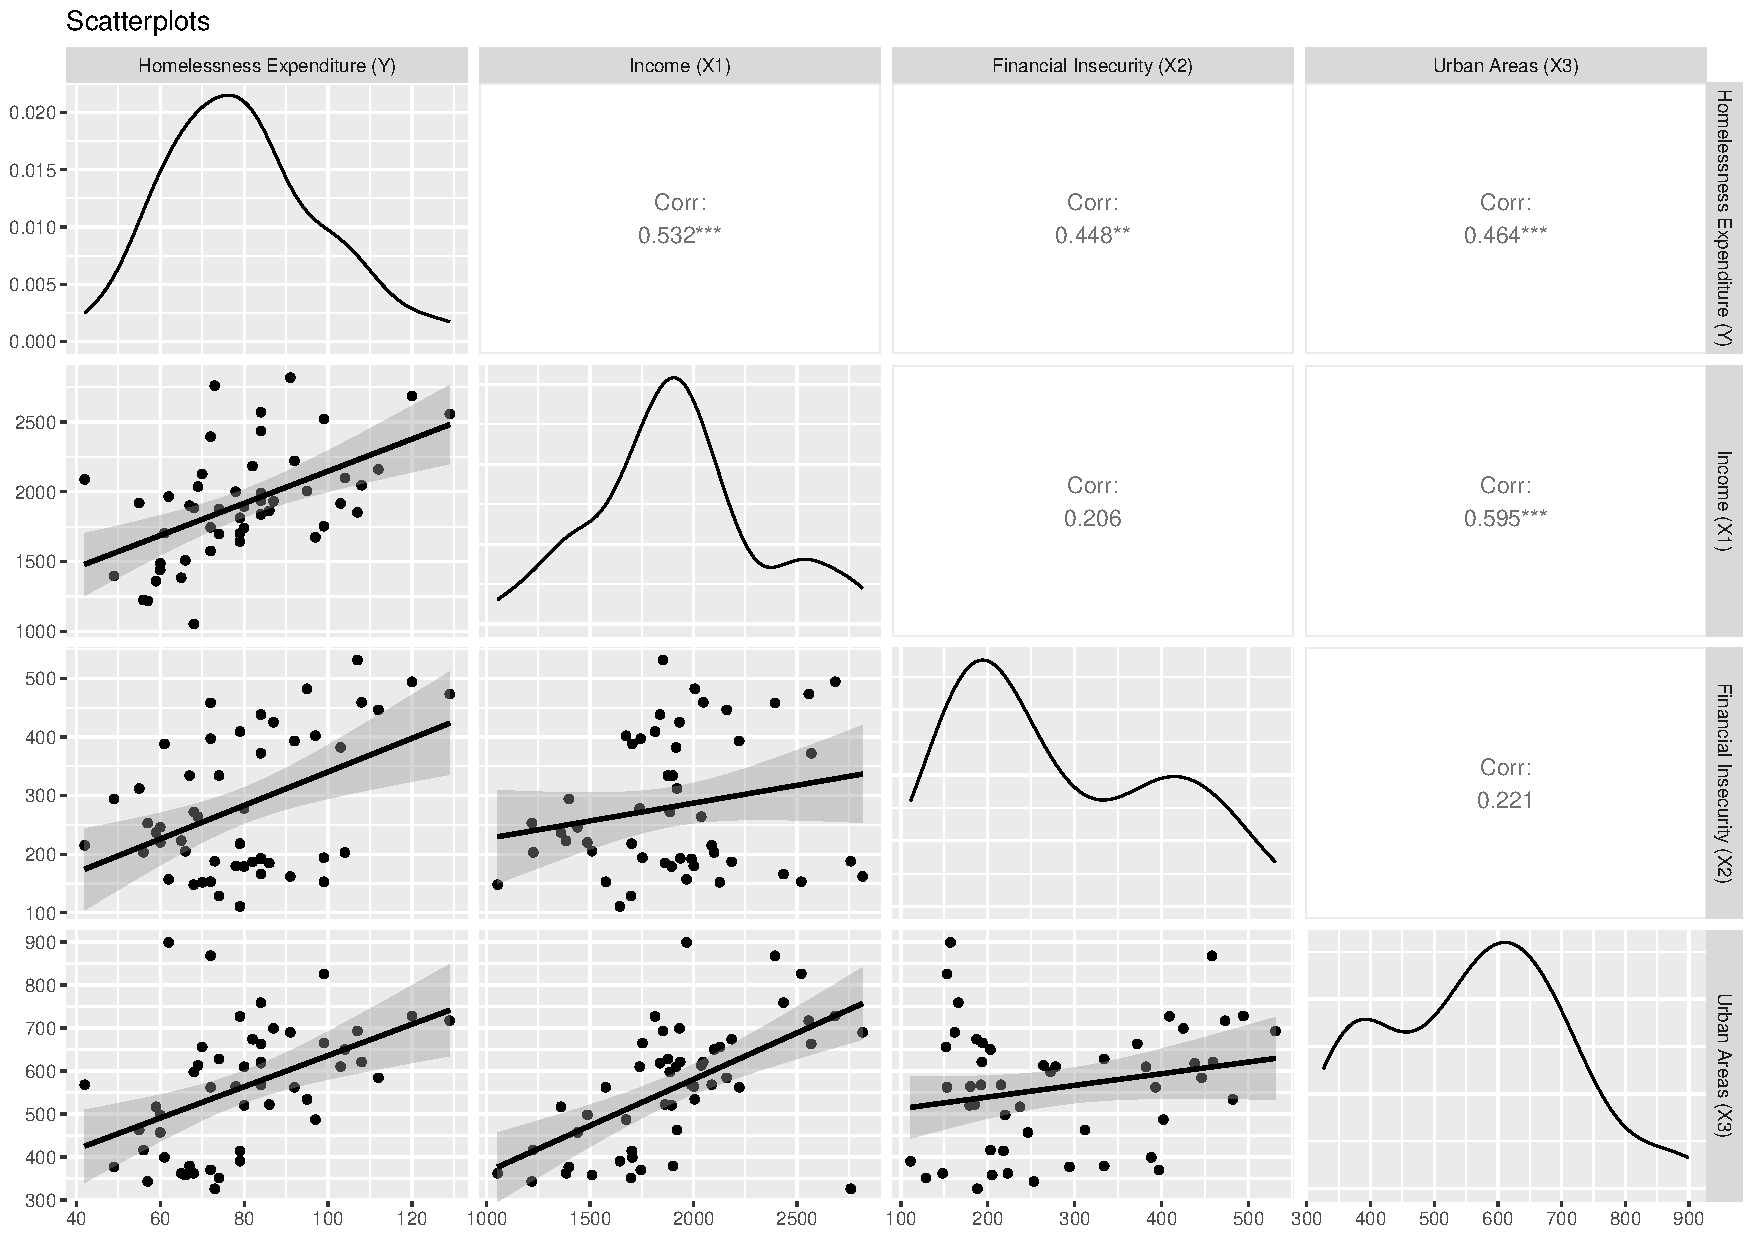
\includegraphics[width=.75\textwidth]{Rplot11.pdf}
\end{figure}

\noindent Expenditure on addressing homelessness (Y) has moderate positive correlations with the variables X1, X2 and X3. Expenditure on homelessness and per capita personal income is the strongest positive correlation between Y and another variable, with a correlation coefficient of .532. The variables X2 and X3 have slightly lower correlation coefficients of .448 and .464 respectively. 
\noindent As there is a positive correlation between Y and the X1, X2 and X3 variables, we can say that as expenditure in addressing homelessness increases, income per capita, number of financially insecure people, and number of people living in urban areas also increase. These correlations are statistically significant to varying levels, as indicated by the *** and ** displayed by the correlation coefficients. The correlation between Y and X1 and Y and X3 is significant to the .001 level, and to .01 between the Y and X2 variables. This indicates that the correlations among Y and the X1, X2 and X3 variables are unlikely to be a result of random chance, and likely indicate an some kind of underlying relationship. \\

\noindent Regarding the correlations between the variables X1, X2 and X3; income per capita and number of financially insecure people are weakly positively correlated. The number of people living in urban areas and number of financially insecure people are also weakly correlated. \\

\noindent The variables per capita personal income and number of people living in urban areas have a moderate positive correlation. This is the strongest overall correlation, with a correlation coefficient of .595. This could create potential issues in isolating the relationship between expenditure on addressing homelessness, and the two correlated variables. For example, if a linear regression was run with Y as the outcome variable and X1, X2 and X3 as the predictor variables, the correlation between X1 and X3 would create problems of multicollinearity. \\
\item
Please plot the relationship between \emph{Y} and \emph{Region}? On average, which region has the highest per capita expenditure on housing assistance?
\lstinputlisting[language=R, firstline=81, lastline=81]{PS01_EL_LA.R}  
\lstinputlisting[language=R, firstline=86, lastline=98]{PS01_EL_LA.R}  
\noindent To compare each region in a graph I created a box plot. In order to have each of the regions show up in separate boxes I used the as.factor code. I also used the stat summary function make the mean expenditure of each reason visible from the graph.  \\
\begin{figure}[h!]\centering
	\caption{\footnotesize Expenditure on Addressing Homelessness by Region.}
	\label{fig:plot_1}
	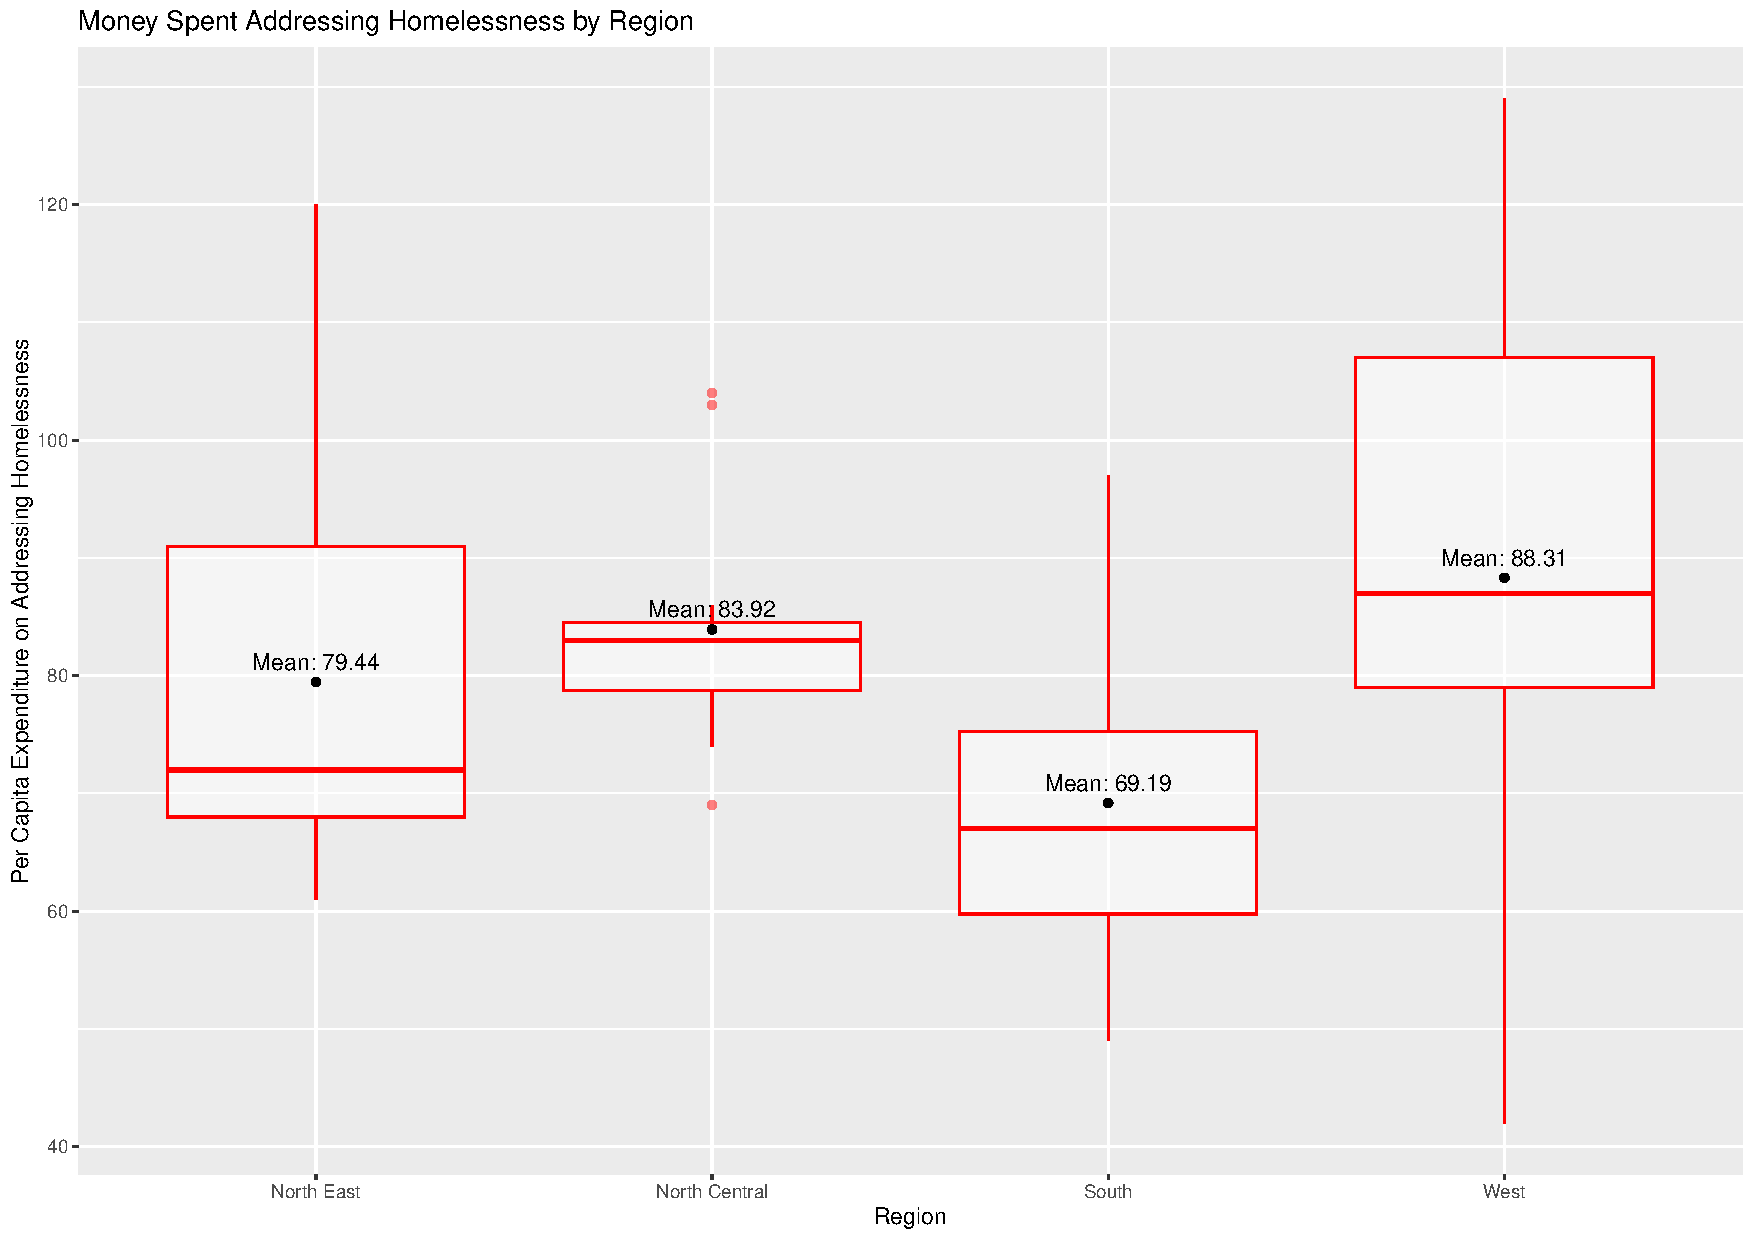
\includegraphics[width=.6\textwidth]{Rplot03.pdf}
\end{figure}

\noindent From the box plot, we can see that the West has the highest expenditure per capita on housing assistance with a mean of 88.31 spent, followed by the North Central with a mean of 83.92, the North East with a mean of 79.44, and the South with a mean of 69.19. From the box plot we can also see that the West had the largest inter-quartile range of the regions, as well as the largest range between the maximum and minimum values. The median was relatively similar to the mean in all regions except the North East where the gap was more pronounced. \\
\vspace{.5cm}
\item
Please plot the relationship between \emph{Y} and \emph{X1}? Describe this graph and the relationship. Reproduce the above graph including one more variable \emph{Region} and display different regions with different types of symbols and colors.
\lstinputlisting[language=R, firstline=101, lastline=107]{PS01_EL_LA.R} 
\noindent To investigate the relationship between Y and X1 I used ggplot to create a scatterplot with a line of best fit. \\

\begin{figure}[h!]\centering
	\caption{\footnotesize Expenditure on Addressing Homelessness and Income.}
	\label{fig:plot_1}
	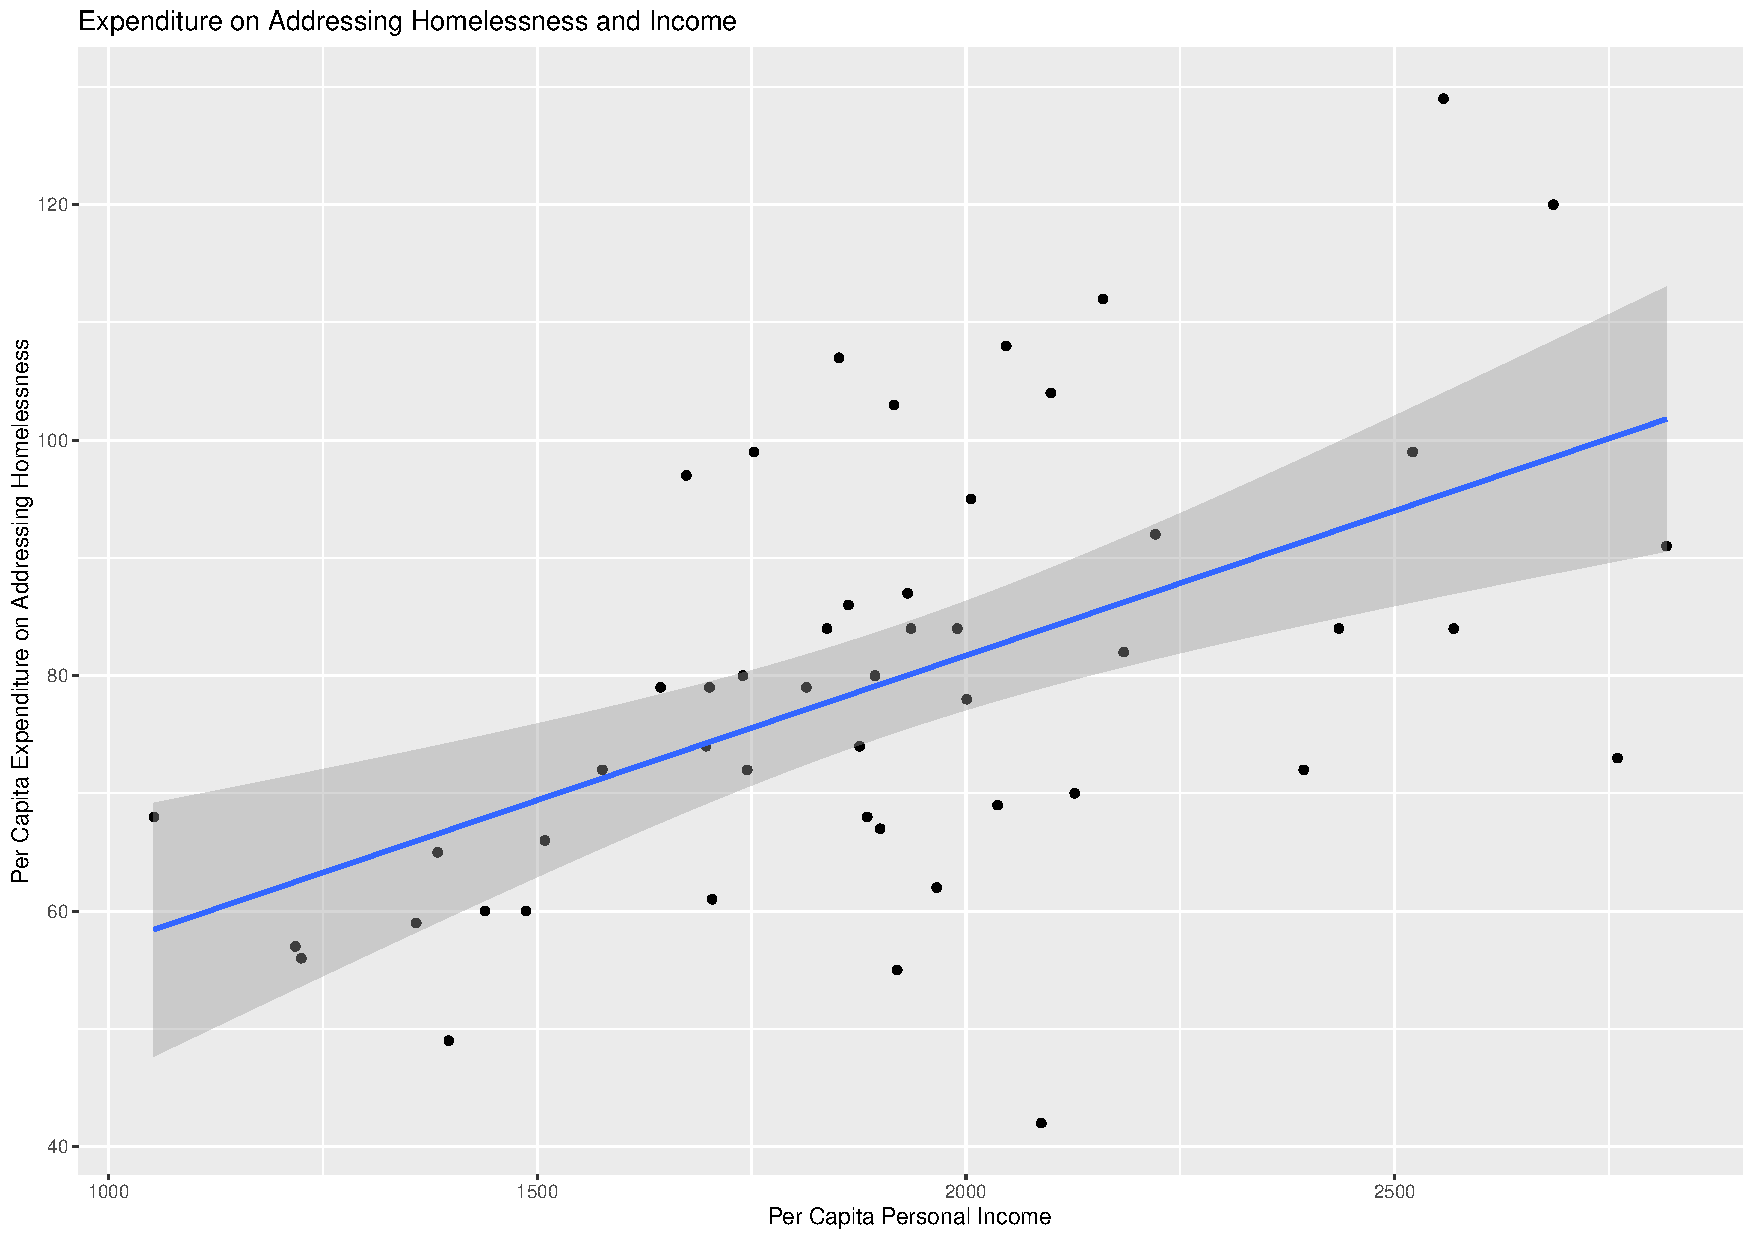
\includegraphics[width=.75\textwidth]{Rplot08.pdf}
\end{figure}
\noindent In the plot we can see that there is a moderately positive correlation between expenditure on addressing homelessness and per capita personal income. This means that as expenditure on addressing homelessness increases, so does per capita personal income. This correlation indicates that there may be some underlying relationship between the variables, but does not imply that the relationship is causal in nature. \\
\lstinputlisting[language=R, firstline=110, lastline=125]{PS01_EL_LA.R}  
\lstinputlisting[language=R, firstline=128, lastline=144]{PS01_EL_LA.R}  
\noindent To reproduce the graph with region I used the ggplot to use the factorized version of the region variable to determine the colour and shape of each value point on the plot. I also ran a second plot in which a line of best fit is present for each of the regions to more clearly differentiate between them. \\

\begin{figure}[h!]\centering
	\caption{\footnotesize Expenditure on Addressing Homelessness and Income by Region.}
	\label{fig:plot_1}
	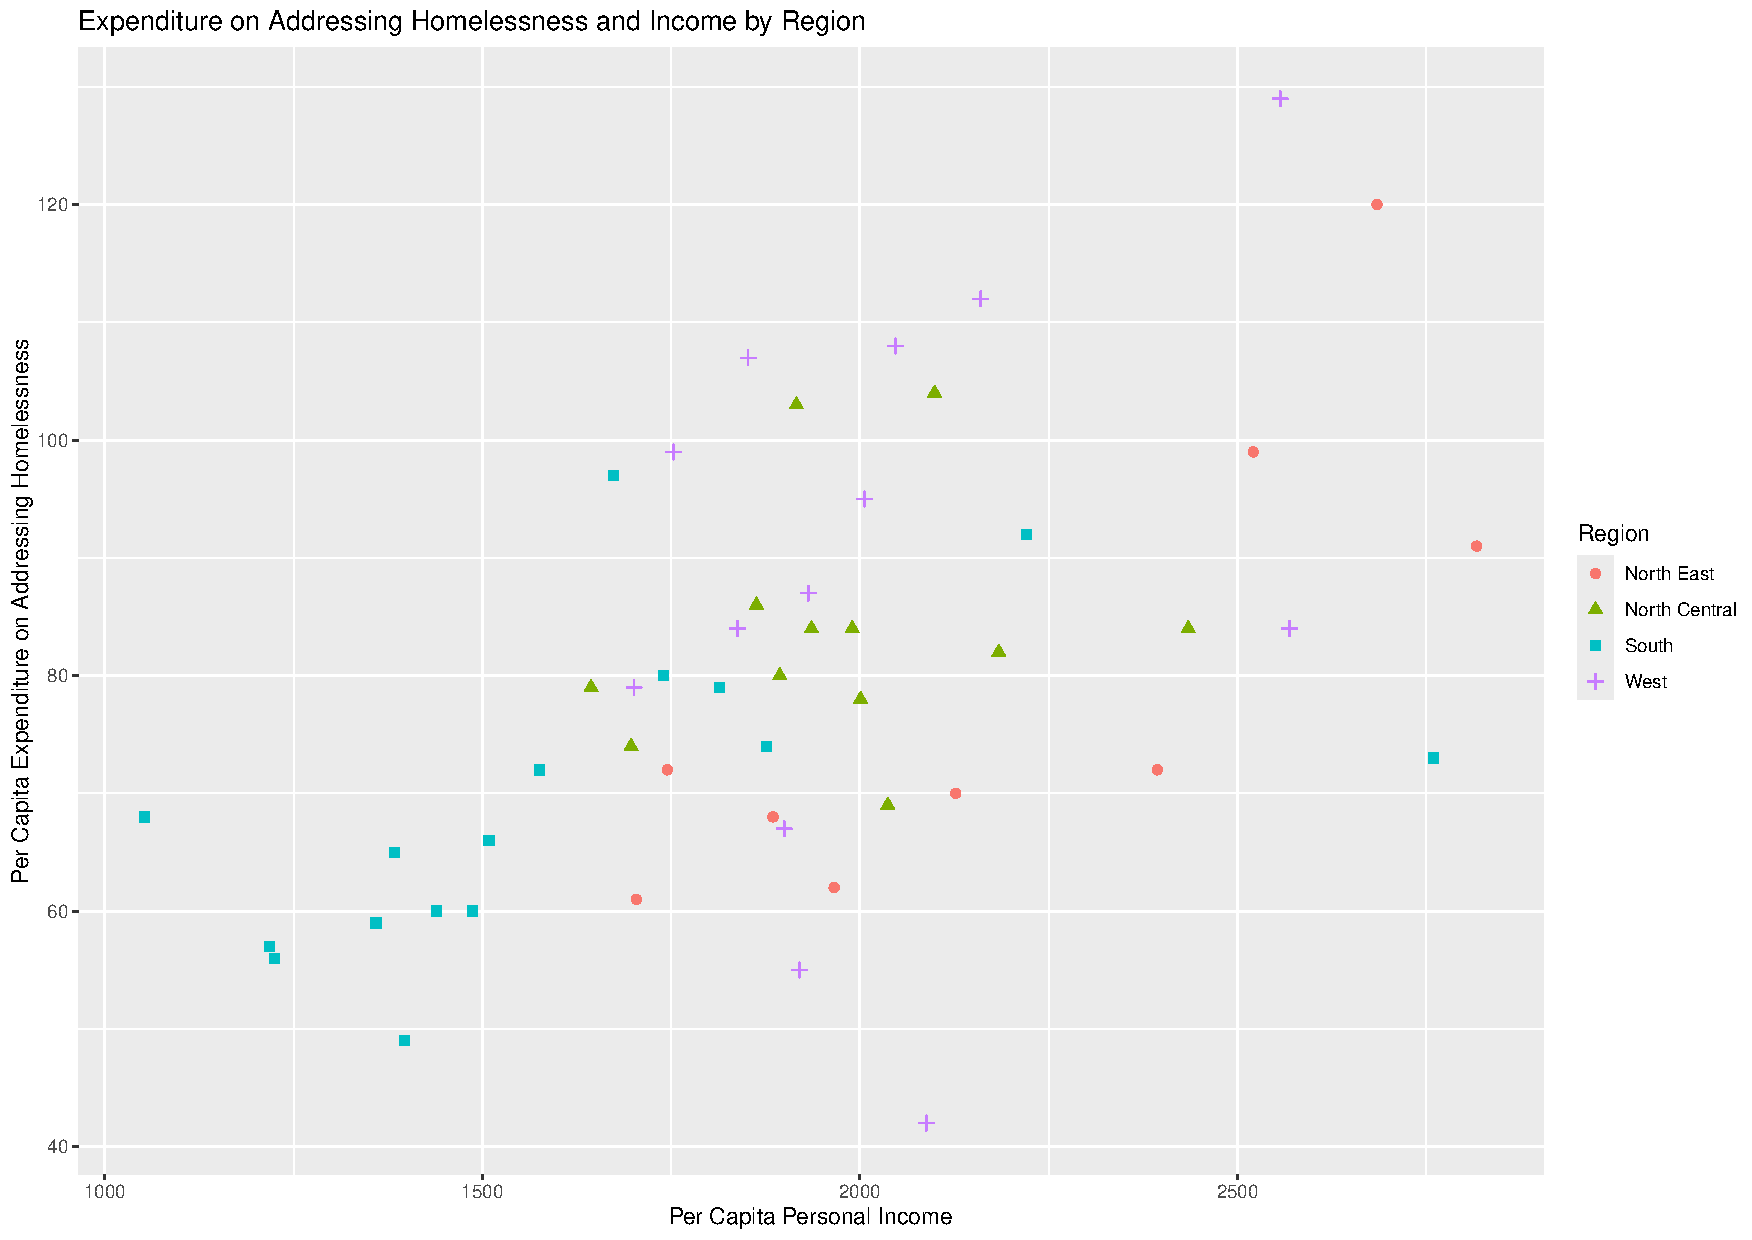
\includegraphics[width=.75\textwidth]{Rplot09.pdf}
\end{figure}
\begin{figure}[h!]\centering
	\caption{\footnotesize   Expenditure on Addressing Homelessness and Income by Region with Line of Best Fit.}
	\label{fig:plot_1}
	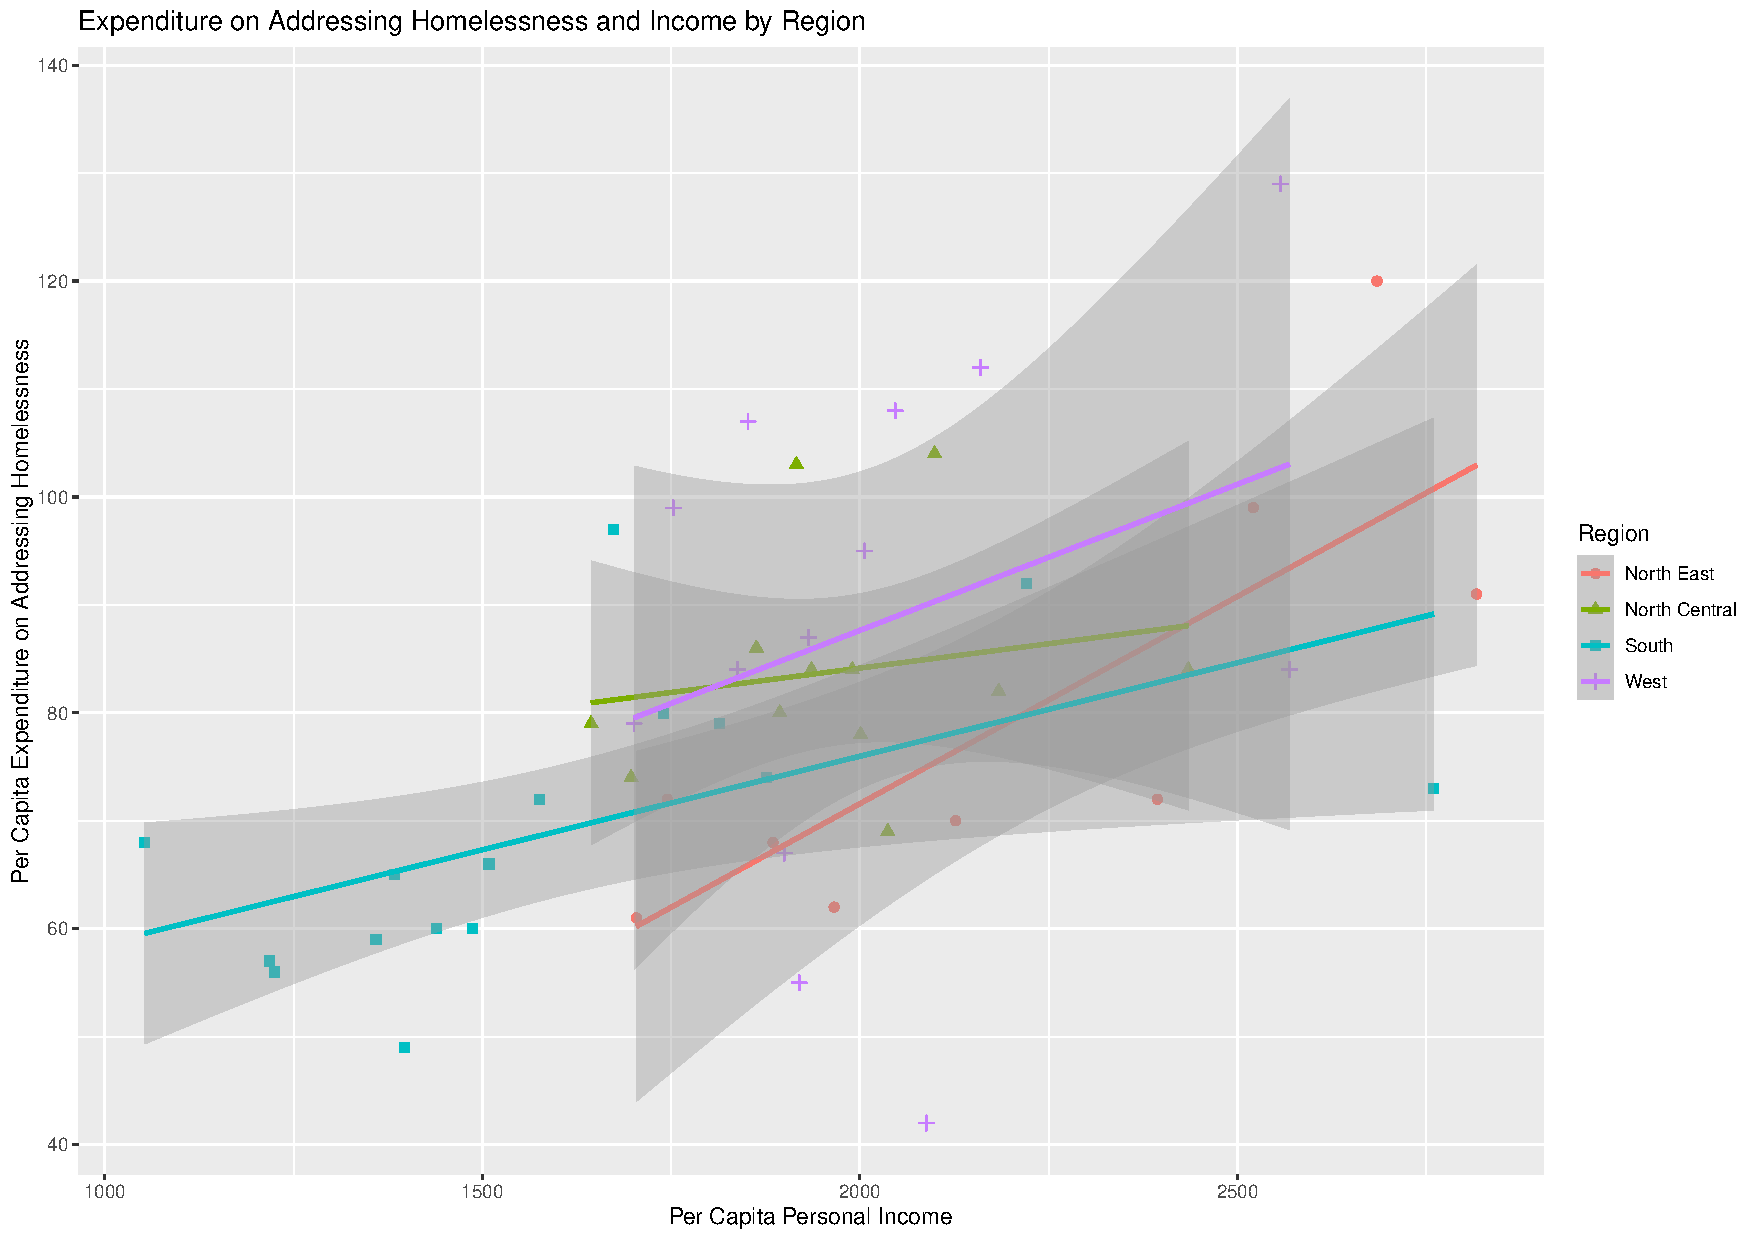
\includegraphics[width=.75\textwidth]{Rplot10.pdf}
\end{figure}

\noindent From the plots we can see that in each region there moderately positive correlation between expenditure on addressing homelessness and income. This is true in each of the four regions, which are all have positive correlations between expenditure on addressing homelessness and per capita income. However the strength of the relationship varies slightly depending on the region, with the North East having the strongest positive correlation of the 4 regions and the North Central having the weakest. We can also see from the plot that the South have the widest range of per capita personal income, while the other four regions have a relatively more concentrated spread of income. \\

\end{itemize}

\newpage

	\section*{References}
	
\noindent GeeksforGeeks. (2021, June 27). Draw Boxplot with Mean in R. GeeksforGeeks. \\
\noindent https://www.geeksforgeeks.org/r-language/draw-boxplot-with-mean-in-r/ \\

\noindent GeeksforGeeks. (2024, July 23). Create a matrix of scatterplots (pairs() equivalent) in GGPLOT2. 
GeeksforGeeks.https://www.geeksforgeeks.org/r-language/create-a-matrix-of-scatterplots-pairs-equivalent-in-ggplot2/ \\

\noindent Scatterplot matrix in R: The pairs() function. (2026, June 27). Datanovia.\\ 
\noindent https://www.datanovia.com/learn/data-visualization/r-base/scatterplot-matrix \\

\end{document}
